\chapter{Hamilton-Jacobi equation}
\section{Derivation of the Hamilton-Jacobi equation}
In this final section regarding analytical mechanics we aim to prove and understand the so-called "Hamilton-Jacobi equation", which is the most abstract way of thinking about mechanics. Up to now we defined action as:
\begin{equation}
  S = \int_{t_1}^{t_2}\lagr\brackets{\vec{q},\dvec{q},t} \dd{t}
\end{equation}
Which means that we think about action as a functional. Now we want to express the same quantity as a function of time and to do so, we need to slightly change our definition:
\begin{equation}
  S \defineeq \int_{t_0}^{t}\lagr\brackets{\vec{q},\dvec{q},t} \dd{t}
\end{equation}
We need to remember that the integral of action \underline{must} be calulated along the actual path of the system we are dealing with, but with this definition, in principle, we can obtain $S$ as a function of time. In particular, we want to prove that $S$ is a function of both time and all the $q_{\alpha}$.
\begin{proof}
  The proof for the time dependence is trivial since:
  \begin{equation}
    \dv{S}{t} = \lagr
  \end{equation}
  For the dependence on $q_{\alpha}$ we can imagine to chang the coordinates without changing the actual path and the time:
  \begin{figure}[H]
    \centering
    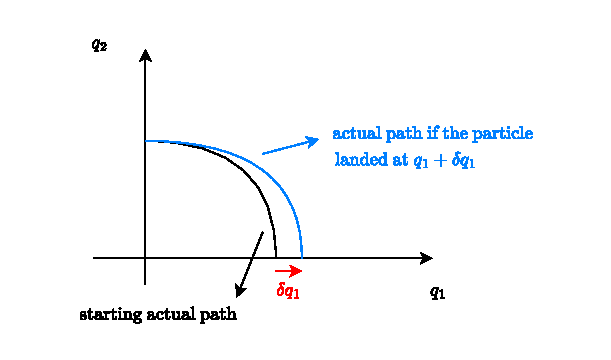
\includegraphics[width=0.6\textwidth]{res/svg/path_change_hamjac.drawio}
    \caption{Path change}
\end{figure}
How does $S$ change for the two trajectories?
\begin{equation}
  \delta S = \int_{t_0}^{t}\cancel{\bigsum_{\alpha}\brackets{\pdv{\lagr}{q_{\alpha}}-\dv{}{t}\pdv{\lagr}{\dot{q}_{\alpha}}}}\delta q_{\alpha} + \int_{t_0}^{t} \dv{}{t} \brackets{\bigsum_{\alpha} \pdv{\lagr}{\dot{q}_{\alpha}}\delta q_{\alpha}}
\end{equation}
We cancel the first part since when we are integrating over the actual path the \eleref\;are true. We then get:
\begin{equation}
  \begin{split}
    \delta S &= \int_{t_0}^{t}\dv{}{t}\brackets{\bigsum_{\alpha} \pdv{\lagr}{\dot{q}_{\alpha}}\delta q_{\alpha}}\\
    &= \bigsum_{\alpha} \pdv{\lagr}{\dot{q}_{\alpha}}\delta q_{\alpha}\bigg|_{t_0}^t =\\
    &= \bigsum_{\alpha} \pdv{\lagr(t)}{\dot{q}_{\alpha}}\delta q_{\alpha}(t) =\\
    &= \bigsum_{\alpha} p_{\alpha} \dd{q_{\alpha}}
  \end{split}
\end{equation}
When we evaluate at $t_0$ the variation is zero since the extremes are fixed. From the final result we have that:
\begin{equation}
  \pdv{S}{q_{\alpha}} = p_{\alpha}
\end{equation}
And so $S$ depends on $q_{\alpha}$
\end{proof}
Now we proved that:
\begin{equation}
  \begin{split} \label{e:dvS}
    \dv{S}{t} &= \bigsum_{\alpha} \pdv{S}{q_{\alpha}}\dot{q}_{\alpha} + \pdv{S}{t} =\\[8pt]
    &= \bigsum_{\alpha} p_{\alpha}\dot{q}_{\alpha} + \pdv{S}{t}
  \end{split}
\end{equation}
But we also know by definition that:
\begin{equation} \label{e:dvS=L}
  \dv{S}{t} = \lagr
\end{equation}
And so combining \eqref{e:dvS} and \eqref{e:dvS=L} we get:
\begin{equation}
  \lagr = \bigsum_{\alpha} p_{\alpha}\dot{q}_{\alpha} + \pdv{S}{t} \implies \underbrace{\lagr - \bigsum_{\alpha} p_{\alpha}\dot{q}_{\alpha}}_{-\hamfun} = \pdv{S}{t}
\end{equation}
And so:
\begin{equation}
  \hamfun (q_{\alpha}, p_{\alpha},t) = -\pdv{S}{t}
\end{equation}
But we also have that $p_{\alpha}$ is the partial time derivative of $S$. From this we can get the \textbf{Hamilton-Jacobi equation}:
\begin{equation} \label{e:hamiltonjacobi}
  \boxed{\hamfun \brackets{q_{\alpha}, \pdv{S}{t},t} = -\pdv{S}{t}}
\end{equation}
This equation is a single partial differential equation that contains all the information of the system. In principle solving this equation makes us able to find the equations of the motion. Unfortunately this equation can be very difficult to solve.
\subsection{Hamilton-Jacobi and canonical transformations}
Let's now think about when we can easily find the equations of the motion in Hamilton's formalism.
\begin{enumerate}
  \item $\hamfun$ is constant and all the coordinates are cyclic.\\
  In this case:
  \begin{equation}
    \dot{p}_{\alpha} = -\pdv{\hamfun}{q_{\alpha}} = 0 \quad \text{(all the momenta are constant)}
  \end{equation}
  And so we have that $p_{\alpha} = Q_{\alpha}$. In this way deriving with respect to the $p_{\alpha}$ just gives us constant numbers and so:
  \begin{equation}
    \dot{q}_{\alpha} = \pdv{\hamfun}{p_{\alpha}} = b_{\alpha} \quad \text{(linear motion of all the coordinates)}
  \end{equation}
  \item $\hamfun$ may be whatever, but all the $q_{\alpha}$ and $p_{\alpha}$ are constant:
  \begin{equation}
    \begin{split}
      \dot{q}_{\alpha} &= 0\\[8pt]
      \dot{p}_{\alpha} &= 0
    \end{split}
  \end{equation}
\end{enumerate}
Let's make an example for the second case.
\subsubsection{Ex. Free particle in 1-D}
Let's suppose that:
\begin{equation}
  \hamfun = \dfrac{p^2}{2m}
\end{equation}
We get:
\begin{equation}
  \begin{split}
    \dot{q} &= \pdv{\hamfun}{p} = \dfrac{p}{m}\\[8pt]
    \dot{p} &= -\pdv{\hamfun}{q} = 0
  \end{split}
\end{equation}
Since $p$ is constant it must be that $p = p_0$ where $p_0$ is the intial value $p(t=0)$. From this it is easy to find the equation of $q$:
\begin{equation}
  q = q_0 + \dfrac{p_0}{m}t
\end{equation}
Let's now make use of this canonical transformation:
\begin{equation}
  \begin{cases}
    Q = q - \dfrac{p}{m}t\\[8pt]
    P = p
  \end{cases}
\end{equation}
Let's check if this transformation is indeed canonical:
\begin{equation}
  \begin{split}
    \pb{Q}{P} &= \brackets{\pdv{Q}{q}\pdv{P}{p} - \pdv{Q}{p}\cancel{\pdv{P}{q}}} = \brackets{\pdv{}{q}\brackets{q - \dfrac{p}{m}t}\pdv{}{p}\brackets{p}}= 1\\
    \pb{Q}{Q} &= \brackets{\pdv{Q}{q}\pdv{Q}{p} - \pdv{Q}{p}\pdv{Q}{q}} = \\
    &= -\dfrac{t}{m} - \brackets{-\dfrac{t}{m}} = 0\\
    \pb{P}{P} &= \brackets{\cancel{\pdv{P}{q}}\pdv{P}{p} - \pdv{P}{p}\cancel{\pdv{P}{q}}} = 0
  \end{split}
\end{equation}
Thus, the transformation satisfies the canonical Poisson bracket relations.\\
We can also try to find a generating function. Since $p = P$ we cannot use a function of the type $F(p,P)$ since the variables wouldn't be independent. Let's choose a first type function:
\begin{equation}
  \begin{split}
    p &= \pdv{F_1}{q}\\[8pt]
    P &= -\pdv{F_1}{Q}
  \end{split}
\end{equation}
We also knwo that the new Lagrangian will be:
\begin{equation}
  \begin{split}
    \lagr &= \tilde{\lagr} + \dv{F_1}{t}\\[8pt]
    p\dot{q} - \hamfun &= P\dot{Q} - \tilde{\hamfun} + \dv{F_1}{t}
  \end{split}
\end{equation}
And so substituting the equations of the transformation:
\begin{equation}
  \begin{split}
    p\dot{q} - \hamfun &= p \dv{}{t}\brackets{Q + \dfrac{p}{m}t} - \dfrac{p^2}{2m} =\\
    &= p\dot{Q} + \dfrac{p\dot{p}}{m}t + \dfrac{p^2}{m} - \dfrac{p^2}{2m} =\\
    &= P\dot{Q} + \dfrac{p\dot{p}}{m}t + \dfrac{p^2}{2m}=\\
    &= P\dot{Q} + \dv{}{t}\bbrackets{\underbrace{\dfrac{p^2}{2m}t}_{F_1}} + \underbrace{0}_{\tilde{\hamfun}}
  \end{split}
\end{equation}
From the transformation equations we have:
\begin{equation}
  F_1 = \dfrac{p^2}{2m}t = \dfrac{m\cancel{^2}(q-Q)^2}{2\cancel{m} t\cancel{^2}}\cancel{t} = \dfrac{m(q-Q)^2}{2t}
\end{equation}
We can verify that this function is actually the action. We know that this must be true:
\begin{equation}
  \begin{split}
    \cancel{\tilde{\hamfun}} - \hamfun &= \pdv{F_1}{t}\\
    \hamfun &= -\pdv{F_1}{t}\\
  \end{split}
\end{equation}
Substituting the functional form we got for $F_1$:
\begin{equation}
  -\pdv{F_1}{t} = -\pdv{}{t}\brackets{\dfrac{m(q-Q)^2}{2t}} = \dfrac{m(q-Q)^2}{2t^2} = \dfrac{p^2}{2m}
\end{equation}
And so this transformation is valid. Now we also notice that we actually wrote the \hamjacref\;equation for $F_1$ and so $F_1$ is indeed the action.
\subsubsection{General statement}
From this example we can try to find a more general approach. In particular, we start from the old coordinates and we want:
\begin{equation}
  \begin{split}
    \begin{Bmatrix}
      q_{\alpha}\\
      p_{\alpha}
    \end{Bmatrix} \longrightarrow
    \begin{Bmatrix}
      Q_{\alpha}\\
      P_{\alpha}
    \end{Bmatrix}\\
    \text{s.t.} \quad \dot{Q}_{\alpha} = 0, \dot{P}_{\alpha} = 0
  \end{split}
\end{equation}
In this way the new coordinates are just numbers:
\begin{equation}
  \begin{split}
    Q_{\alpha} = b_{\alpha}\\
    P_{\alpha} = a_{\alpha}
  \end{split}
\end{equation}
And also the new Hamiltonian must be zero since:
\begin{equation}
  \begin{cases}
    \dot{Q}_{\alpha} = \pdv{\tilde{\hamfun}}{P_{\alpha}} = \pdv{\tilde{\hamfun}}{a_{\alpha}} = 0\\[8pt]
    \dot{P}_{\alpha} = -\pdv{\tilde{\hamfun}}{Q_{\alpha}} = -\pdv{\tilde{\hamfun}}{b_{\alpha}} = 0
  \end{cases}
\end{equation}
Let's try to find the generating function of this transformation by supposing that it is a type 2 function $F_2(\vec{q},\vec{P},t)$.
From the theory of canonical transformations we know that:
\begin{equation} \label{propertiesf2}
  \begin{split}
    \cancel{\tilde{\hamfun}} - \hamfun &= \pdv{F_2}{t}\\[8pt]
    p_{\alpha} &= \pdv{F_2}{q_{\alpha}}\\[8pt]
    Q_{\alpha} &= \pdv{F_2}{P_{\alpha}}
  \end{split}
\end{equation}
From the first equation:
\begin{equation}
  \hamfun \brackets{q_{\alpha}, p_{\alpha},t}= -\pdv{F_2}{t}
\end{equation}
But from the second equation we get:
\begin{equation}
  \hamfun \brackets{q_{\alpha}, \pdv{F_2}{q_{\alpha}},t}= -\pdv{F_2}{t}
\end{equation}
Again this is the \hamjacref\;equation and the function $F_2$ is called \textbf{Hamilton's principal function} and is denoted with $S$:
\begin{equation}
  \hamfun \brackets{q_{\alpha}, \pdv{S}{q_{\alpha}},t}= -\pdv{S}{t}
\end{equation}
As we anticipated this equation has some fundamental properties:
\begin{itemize}
  \item It is 1 first order PDE
  \item It has $n+1$ integration constant, but one is actually trivial since it is just a generic number and we can ignore it. Thus, we have $n$ "true" integration constants
  \item $S$ is of the second type $S = S(\vec{q},\vec{P},t)$
\end{itemize}
From these properties we know that $S$ depends on the $n$ integration constants $k_{\alpha}$ which depend on the various $P_{\alpha}$. We can identify all the integration constants as the values of $P_{\alpha} = a_{\alpha}$ and so $k_{\alpha} = a_{\alpha}$.\\
Now we want to find the equations of $q_{\alpha}$ and $p_{\alpha}$ as functions of the constant numbers $b_{\alpha}$ and $a_{\alpha}$. Going back to \eqref{propertiesf2}:
\begin{equation}
  b_{\alpha} = Q_{\alpha} = \pdv{S}{P_{\alpha}}
\end{equation}
And so $b_{\alpha} = b_{\alpha}(\vec{q},\vec{a},t)$. Inverting this equation we have $q_{\alpha} = q_{\alpha}(\vec{b},\vec{a},t)$. But we already knew that $p_{\alpha} = p_{\alpha}(\vec{q},\vec{a},t)$ and so substituting the equation found for $q_{\alpha}$ we have:
\begin{equation}
  \begin{split}
    q_{\alpha} = q_{\alpha}(\vec{b},\vec{a},t)\\[8pt]
    p_{\alpha} = p_{\alpha}(\vec{b},\vec{a},t)
  \end{split}
\end{equation}
Which is what we wanted. Now to determine what the constants are we set the intial conditions, which correspond to when $t=0$:
\begin{equation}
  \begin{cases}
    q_{\alpha}(t=0)= q_{\alpha 0} = q_{\alpha}(\vec{b},\vec{a},0)\\[8pt]
    p_{\alpha}(t=0)= p_{\alpha 0} = p_{\alpha}(\vec{b},\vec{a},0)
  \end{cases}
\end{equation}
By inverting those equations we get the integration constants:
\begin{equation}
  \begin{cases}
    a_{\alpha} = a_{\alpha}(\vec{q}_0,\vec{p}_0,0)\\[8pt]
    b_{\alpha} = b_{\alpha}(\vec{q}_0,\vec{p}_0,0)
  \end{cases}
\end{equation}
Since we found that the equations of the motion only depend on the constants $a_{\alpha}$ and $b_{\alpha}$ we have:
\begin{equation}
  \begin{cases}
    q_{\alpha} = q_{\alpha}(\vec{q}_0,\vec{p}_0,t)\\[8pt]
    p_{\alpha} = p_{\alpha}(\vec{q}_0,\vec{p}_0,t)
  \end{cases}
\end{equation}
This is the final solution. In particular this last equation finally makes us understand that the equations of the motion only depend on the initial conditions.
\subsection{Hamilton-Jacobi and the Schrödinger equation}
It is possible to prove that the Schrödinger equation is the quantum counterpart of the classical Hamilton-Jacobi equation. In particular:
\begin{equation}
  \text{Schrödinger equation} \quad \xrightarrow{\text{classical limit}} \quad \text{Hamilton-Jacobi equation}
\end{equation}
For 1 particle:
\begin{equation}
  \begin{split}
    \hamfun &= \dfrac{p^2}{2m} + V\\[8pt]
    \hat{H} &= -\dfrac{\hbar^2}{2m} \lap + V \rightarrow -\dfrac{\hbar^2}{2m} \pdv[2]{}{q} + V
  \end{split}
\end{equation}
Now let:
\begin{equation}
  \Psi(q,t) = \efunction^{(i/ \hbar) S(q,t)}
\end{equation}
Where $S = a + ib$ is a complex number. Using Schrödinger equation, for the time derivative part we have:
\begin{equation}
  \begin{split}
    \pdv{\Psi}{t} &= \efunction^{(i/ \hbar) S} \dfrac{i}{\hbar}\pdv{S}{t}\\[8pt]
    i\hbar\pdv{\Psi}{t} &= -\pdv{S}{t} \Psi
  \end{split}
\end{equation}
For the part with the Hamiltonian operator we have:
\begin{equation}
  \begin{split}
    \pdv{\Psi}{t} &= \brackets{\dfrac{i}{\hbar}}\efunction^{(i/ \hbar) S} \pdv{S}{q}\\[8pt]
    \pdv[2]{\Psi}{t} &= \brackets{\dfrac{i}{\hbar}}^2\efunction^{(i/ \hbar) S}\brackets{\pdv{S}{q}}^2 + \brackets{\dfrac{i}{\hbar}}\efunction^{(i/ \hbar) S} \pdv[2]{S}{q}=\\
    &= \brackets{\dfrac{i}{\hbar}}^2\brackets{\pdv{S}{q}}^2 \Psi + \brackets{\dfrac{i}{\hbar}}\pdv[2]{S}{q} \Psi
  \end{split}
\end{equation}
And so we have:
\begin{equation}
  \begin{split}
    -\pdv{S}{t} \cancel{\Psi} &= \dfrac{\hbar^2}{2m}\brackets{\dfrac{i}{\hbar}}^2\brackets{\pdv{S}{q}}^2 \cancel{\Psi} + \dfrac{\hbar^2}{2m}\brackets{\dfrac{i}{\hbar}}\pdv[2]{S}{q} \cancel{\Psi} + V\cancel{\Psi}\\[8pt]
    -\pdv{S}{t} &= \dfrac{-1}{2m}\brackets{\pdv{S}{q}}^2  + \dfrac{i\hbar}{2m}\pdv[2]{S}{q} + V
  \end{split}
\end{equation}
If we take the limit for $\hbar \rightarrow 0$ we finally get:
\begin{equation}
  \begin{split}
    -\pdv{S}{t} &= \dfrac{1}{2m}\brackets{\pdv{S}{q}}^2  - \cancel{\dfrac{i\hbar}{2m}\pdv[2]{S}{q}} + V\\[8pt]
    -\pdv{S}{t} &= \dfrac{1}{2m}\bbrackets{\underbrace{\pdv{S}{q}}_{p}}^2 + V
  \end{split}
\end{equation}
Which results in the \hamjacref :
\begin{equation}
  \begin{split}
    -\pdv{S}{t} &= \dfrac{p^2}{2m} + V\\[8pt]
    -\pdv{S}{t} &= \hamfun (q, \pdv{S}{q},t)
  \end{split}
\end{equation}
